\subsection{Entropy}
To compute the optimum decision point for the individual principle components, the entropy method is used.
The entropy of the PC's with our ten ciphers is given by equation \ref{eq:entropy}.

\begin{equation}
Entropy(S) = \sum_{i = '0'}^{'9'} -p_i \cdot \log_2(p_i) 
\qquad \because p_i = P(x = i)
\label{eq:entropy}
\end{equation}

To find the best decision point, it is wanted that the entropy of the two resulting systems, when dividing one PC into two, is as low as possible.
This can be represented as sum of entropy for our two resulting datasets, weighted by the relative size of such.
This is given in equation \ref{eq:entropy_datasetdevision}.

\begin{eqnarray}
Entropy = \sum_{i = 1}^{2} \frac{s_i \cdot Entropy(S_i)}{\sum_{k = 1}^{2} s_k} 
\qquad \because S_i \subset S\ and\ s_k = size(S_k)
\label{eq:entropy_datasetdevision}
\end{eqnarray}

When using equation \ref{eq:entropy_datasetdevision} on the first five principle components on the data of 15 people from the class, then figure \ref{fig:entropy_pc5} was gained.

\begin{figure}[H]
\centering
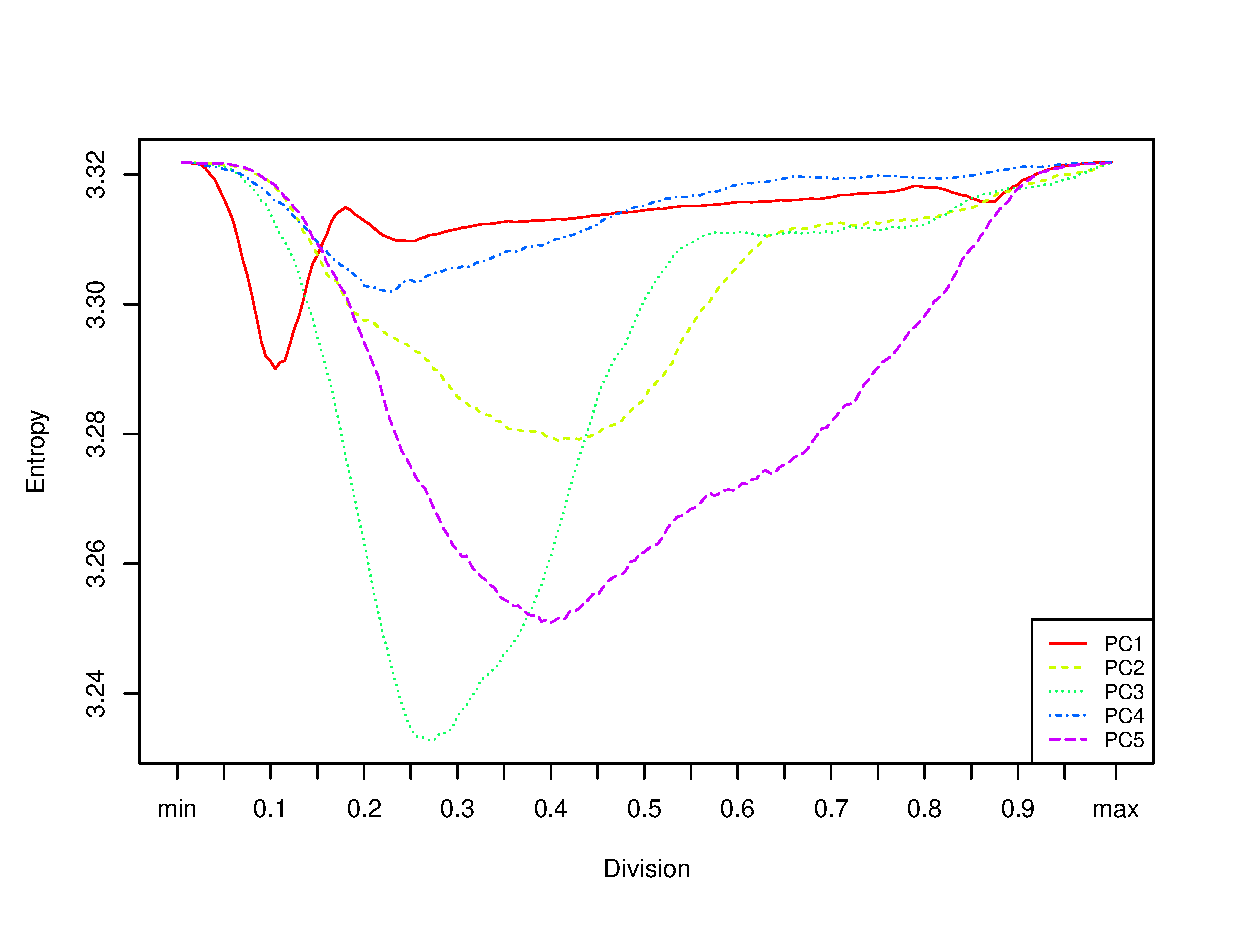
\includegraphics[width = 0.95 \textwidth]{graphics/entropy_pc}
\caption[Variation of the entropy]{Figure showing the variation of the entropy of the dataset when the decision point varies. Computed using equation \ref{eq:entropy_datasetdevision}. The data of the first five principle component.}
\label{fig:entropy_pc5}
\end{figure}


The point of lowest entropy for a principle component was then used as the splitting point to convert the data into binary.
This was done by setting everything below the splitting point to true and the rest false.
This was then done for all principle components on both the test and train set. 
The splitting point for the components in the test set were taken as the splitting point from the same component in the train set.

The optimal decision decision point is shown along with the PC values for PC1 in figure \ref{fig:decision_point}. 
The different data rows represent the ten different characters (from zero to nine).
Here it is clear that if the data is above the split then it is highly unlikely to be a 0.
If the data is below, further investigation is needed.
By removing all unlikely classes the true class must remain.

\begin{figure}[H]
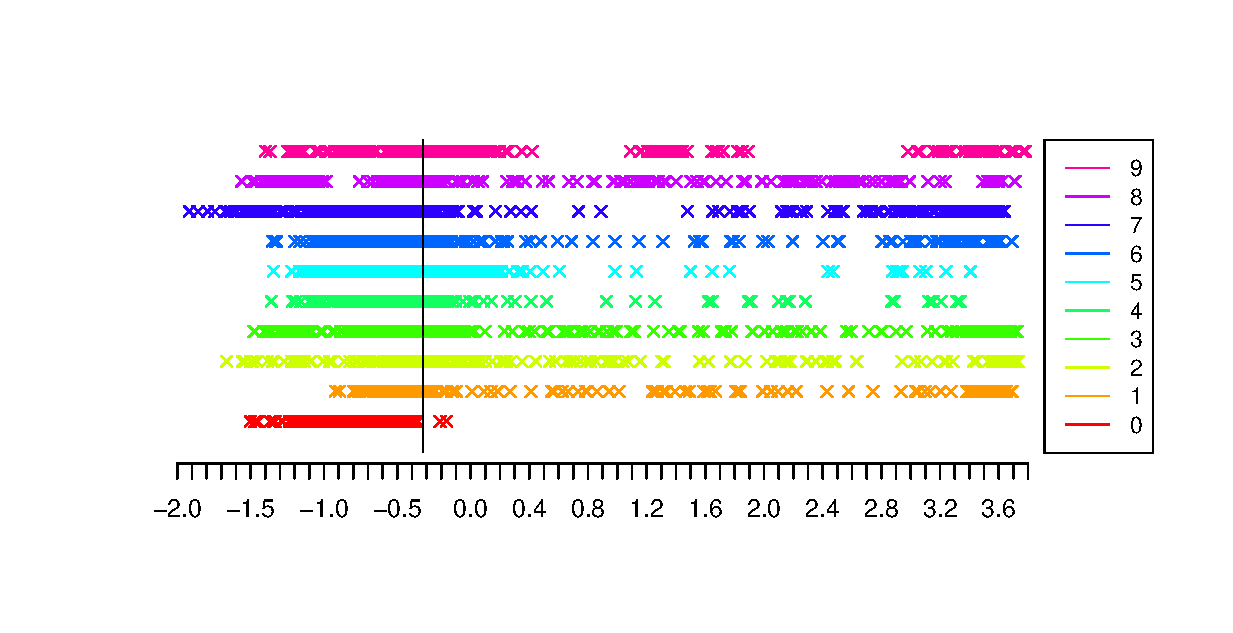
\includegraphics[width = \textwidth]{graphics/decision_seperation}
\caption{Decision point in relation to PC values.}
\label{fig:decision_point}
\end{figure}





